\chapter{Resultados: Dashboards e Indicadores}
\label{cap:resultados}

O \textit{warehouse} descrito no Capítulo~\ref{cap:dw} ganha forma de produto de dados na camada de consumo: cinco páginas analíticas, além de Início e Glossário. Todas leem o banco DuckDB materializado pelo \textit{pipeline} dbt e compartilham filtros globais na barra lateral. Este capítulo corresponde à apresentação do artefato em uso, articulando-se com a fase de avaliação do ciclo DSR.

A organização das páginas segue uma lógica de "visão cidadã": títulos e legendas evitam, quando possível, o uso de jargão contábil; termos técnicos aparecem com explicação no Glossário ou em \textit{tooltips} acionados pelo cursor. Cada página analítica abre um bloco recolhível intitulado "O que você quer descobrir?", que orienta a leitura com perguntas concretas antes de expor gráficos e tabelas. O restante deste capítulo percorre as visualizações principais, descreve os indicadores calculados e contrasta o que o painel permite observar em relação ao Portal da Transparência original.

\section{Visão Geral da Execução Orçamentária}

A leitura consolidada da execução orçamentária distribui-se em duas páginas complementares. A Visão Geral Fiscal responde, em primeiro lugar, se a arrecadação e os pagamentos no recorte filtrado fecham no azul ou no vermelho. Quatro indicadores resumem o recorte: arrecadação, pagamentos, saldo fiscal (diferença entre os dois) e percentual de execução da receita em relação à previsão atualizada. Uma segunda faixa compara a arrecadação e os pagamentos do último mês com os dados disponíveis no filtro de ano. A terceira faixa exibe série mensal de arrecadação \textit{vs.} pagamentos, com eixo vertical em escala logarítmica quando a dispersão de magnitudes exige.

A página Despesas aprofunda os três estágios da despesa pública municipal. No resumo, aparecem valores agregados de empenhado, liquidado e pago, seguidos de razões derivadas dos fatos: percentual liquidado sobre empenhado, percentual pago sobre empenhado e percentual pago sobre liquidado. Esses percentuais não medem execução sobre dotação autorizada, a informação está ausente na fonte, conforme discutido no Capítulo~\ref{cap:dw}, mas indicam em que medida o compromisso empenhado se converteu em saída efetiva de caixa.

\begin{figure}[h]
\begin{center}
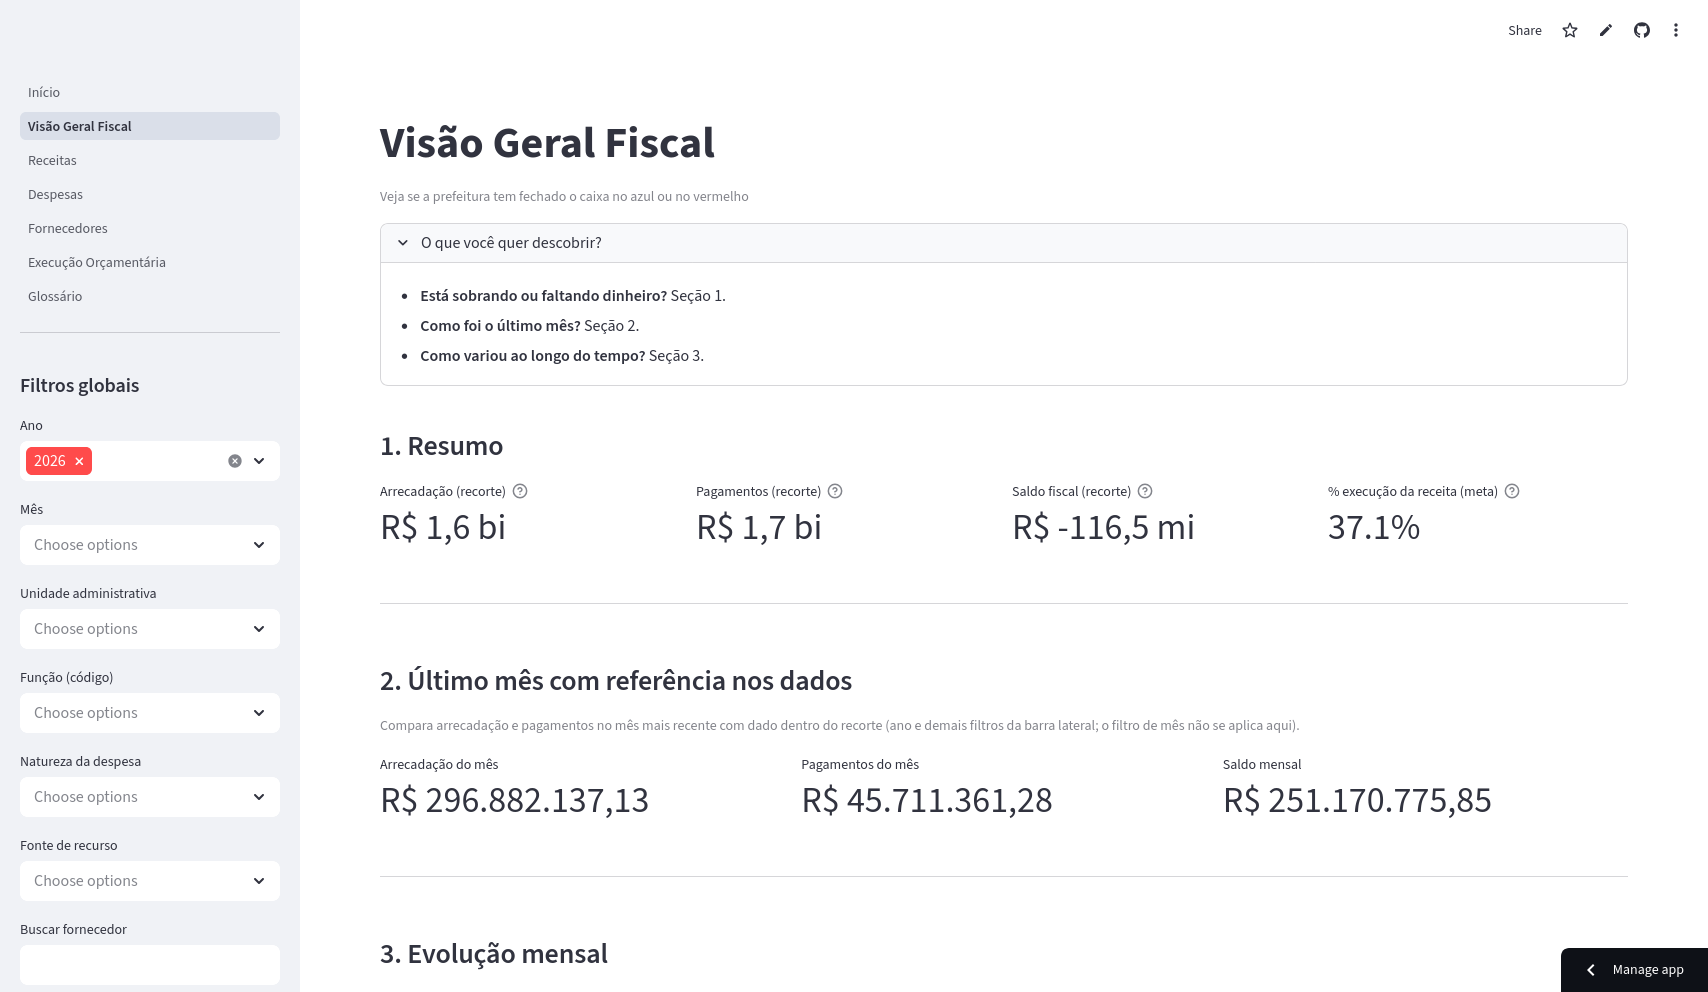
\includegraphics[width=\textwidth]{figs/visao_geral_fiscal_1_2.png}
\caption{Visão Geral Fiscal: resumo do recorte e comparação do último mês (seções 1 e 2).}
\label{fig:visao-geral-fiscal-resumo}
\end{center}
\end{figure}

\begin{figure}[h]
\begin{center}
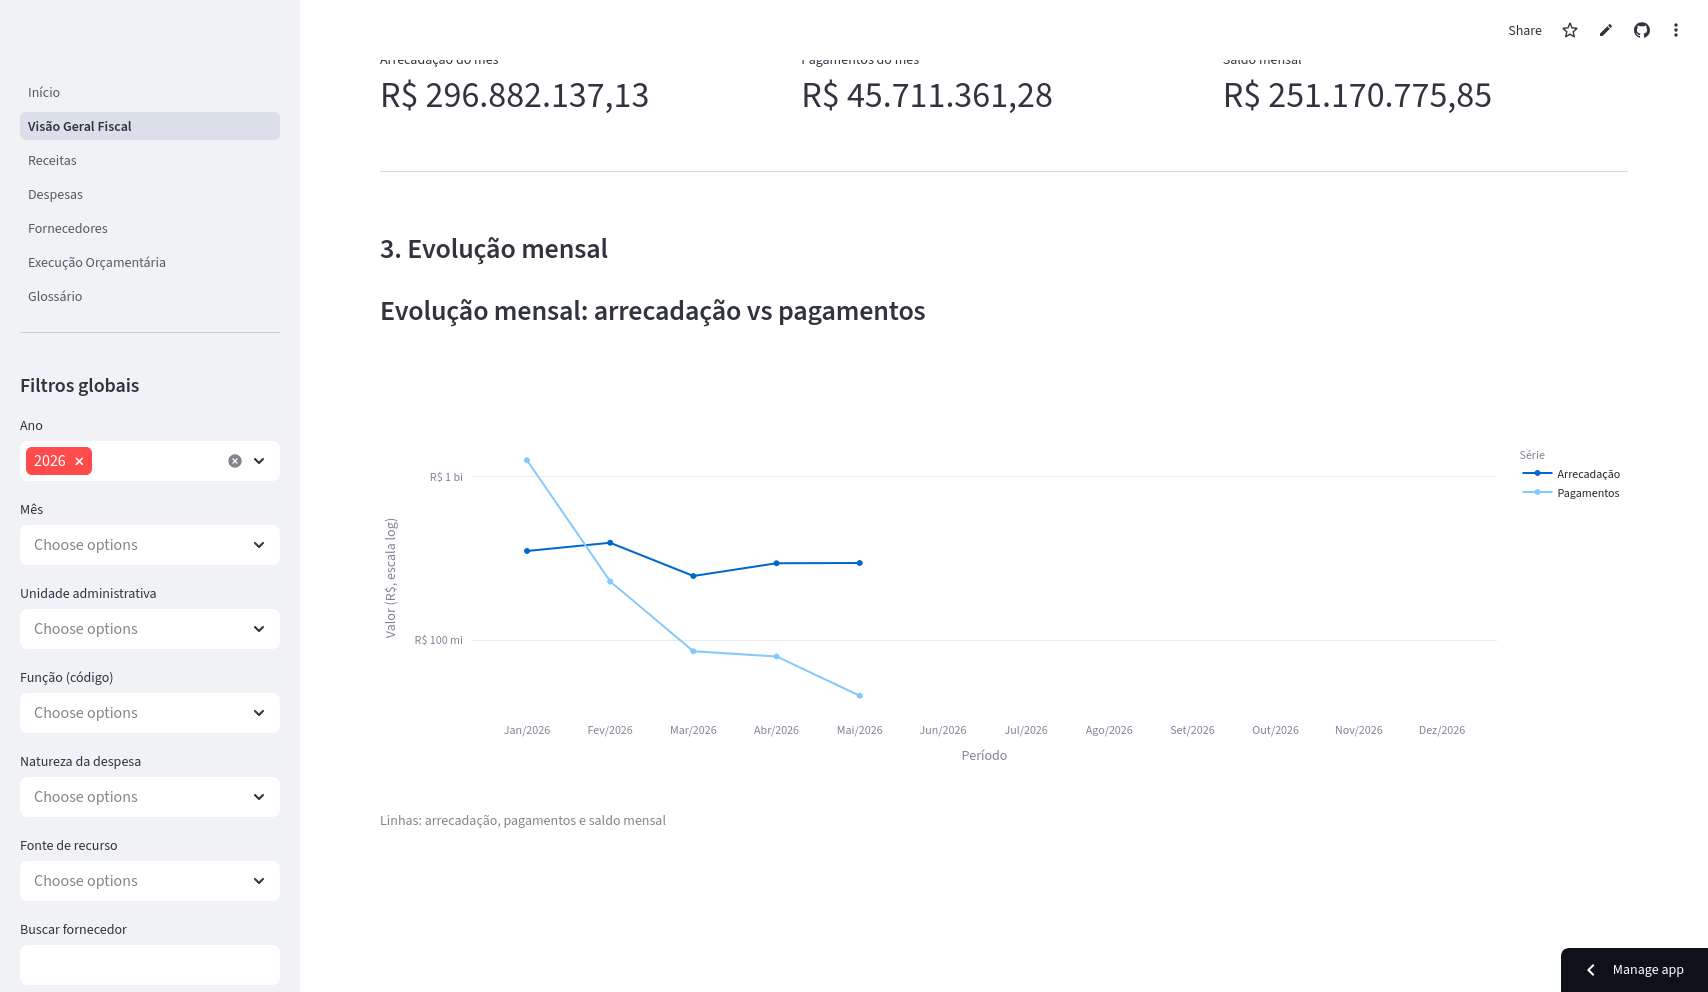
\includegraphics[width=\textwidth]{figs/visao_geral_fiscal_3.png}
\caption{Visão Geral Fiscal: evolução mensal de arrecadação \textit{vs.} pagamentos (seção 3).}
\label{fig:visao-geral-fiscal-evolucao}
\end{center}
\end{figure}

\begin{figure}[h]
\begin{center}
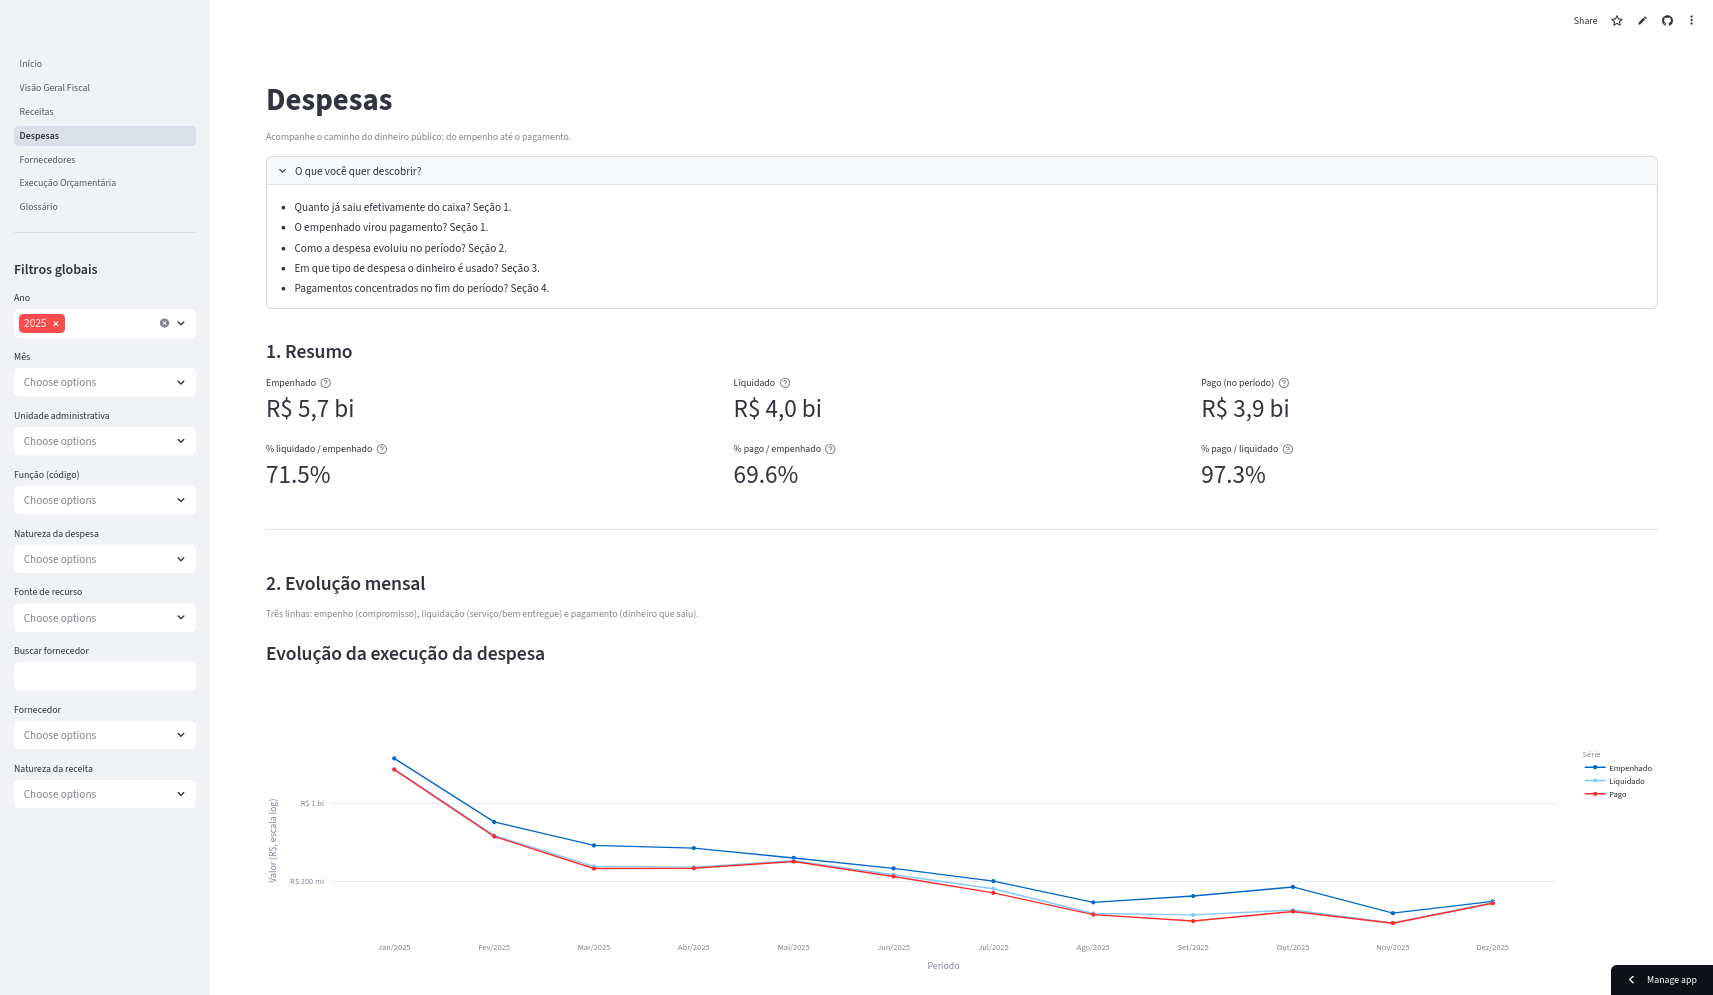
\includegraphics[width=\textwidth]{figs/despesas_1_2.png}
\caption{Despesas: resumo dos estágios da execução e da evolução mensal empenhada, liquidada e paga.}
\label{fig:despesas-resumo-evolucao}
\end{center}
\end{figure}

No portal municipal, receitas e despesas vivem em planilhas distintas, sem cruzamento automático nem série temporal unificada. Empenhado, liquidado e pago aparecem como colunas do relatório mensal, mas comparar estágios ao longo de anos ou filtrar por secretaria exige trabalho manual de consolidação. O painel reduz esse esforço a poucos cliques nos filtros globais e devolve, de imediato, indicadores que antes dependiam de uma planilha montada pelo próprio usuário.

\section{Execução por Função de Governo}

A página Execução Orçamentária desagrega a despesa por órgão executor e por classificação funcional. A primeira seção ordena as unidades administrativas pelos valores empenhados, liquidados e pagos no período, com um gráfico de barras agrupadas das vinte maiores e uma tabela completa ordenada por pagamento. A segunda seção extrai códigos de função e de subfunção da \textit{string} funcional programática publicada no consolidado mensal e faz \textit{join} com \texttt{dim\_funcao} e \texttt{dim\_subfuncao}, alimentadas pela LOA PJF do exercício 2026.

Essa página responde, com ressalvas, à pergunta exemplar da introdução: \textit{"Quanto Juiz de Fora investiu em educação nos últimos três anos?"}. Basta selecionar os anos desejados no filtro global e localizar, na tabela funcional, as linhas cuja função corresponde à educação. A comparação entre exercícios deixa de exigir abrir doze planilhas anuais e alinhar manualmente códigos funcionais programáticos.

\begin{figure}[h]
\begin{center}
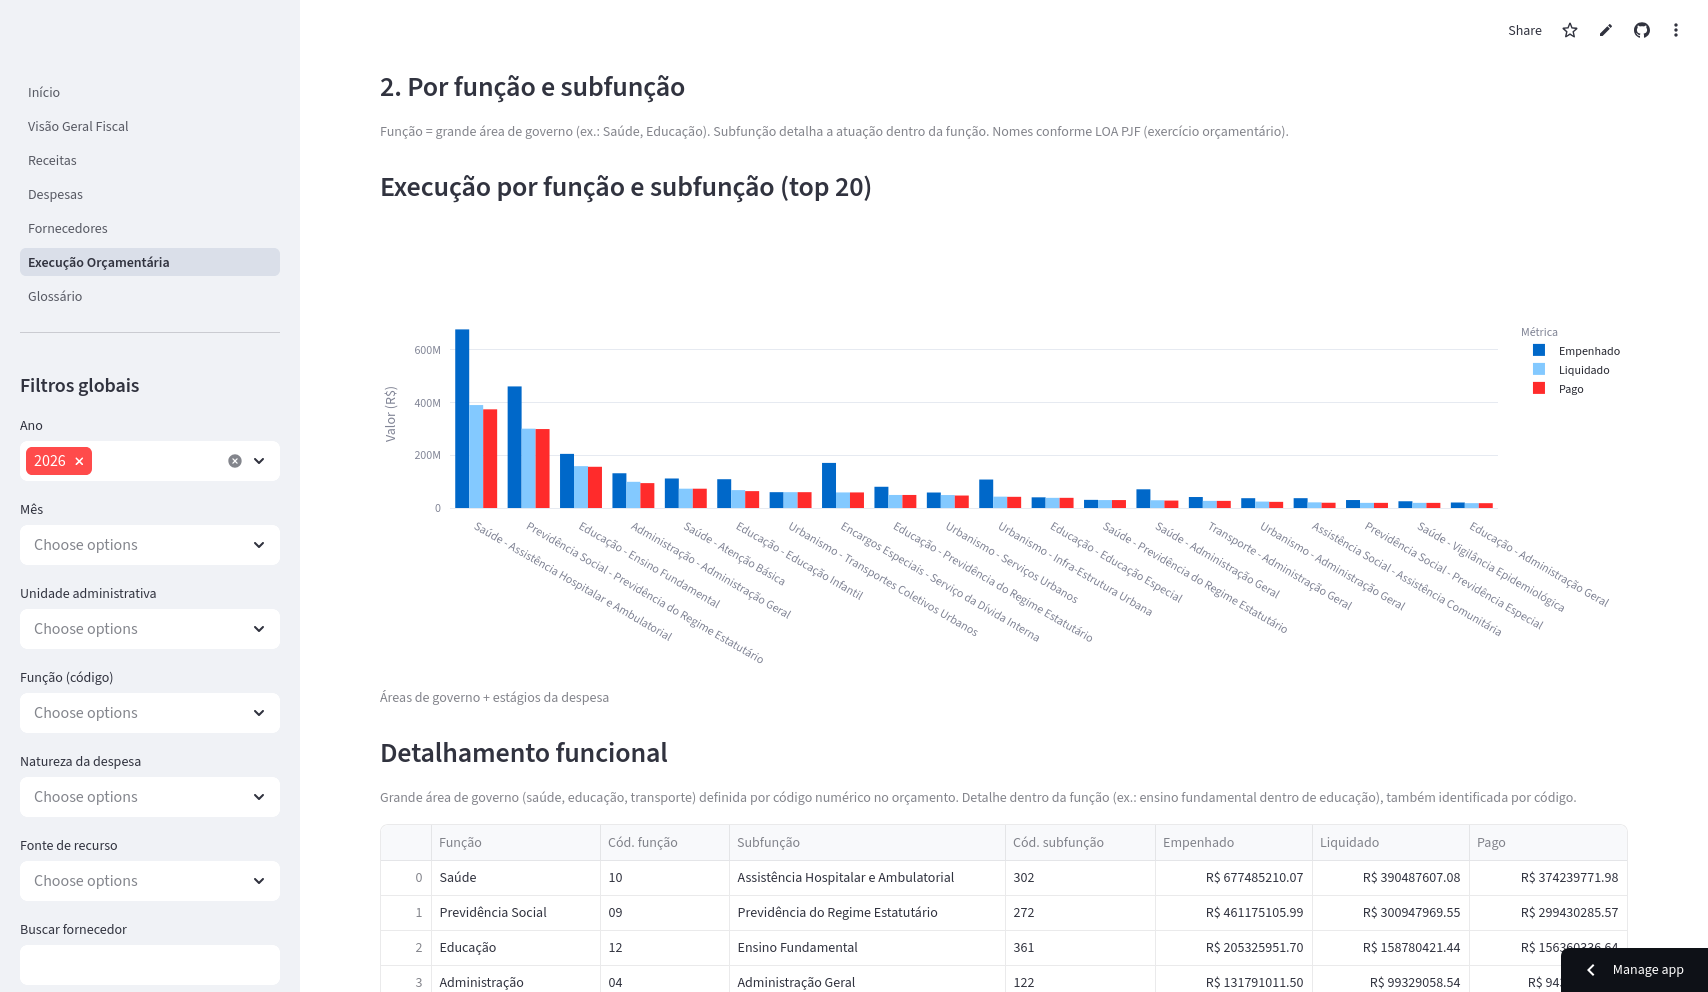
\includegraphics[width=\textwidth]{figs/exec_2.png}
\caption{Execução Orçamentária por função e subfunção: gráfico das vinte maiores combinações e tabela funcional.}
\label{fig:execucao-funcao}
\end{center}
\end{figure}

\section{Concentração de Fornecedores}

A página Fornecedores trata da questão do favorecimento e da concentração de recursos. O resumo destaca o maior favorecido do ranking, a base total de pagamentos considerada e a parcela acumulada pelos cinco primeiros do ranking. A seção de concentração exibe um gráfico horizontal com os vinte maiores pagamentos e uma tabela com valor pago, quantidade de empenhos distintos e participação percentual no total do recorte. A terceira seção permite escolher um fornecedor e visualizar a evolução mensal dos pagamentos a ele, o que é útil para verificar se um contrato pontual distorce o ranking ou se há recebimento recorrente ao longo do tempo.

O portal publica o favorecido e o valor pago na planilha de despesa, mas não calcula a participação relativa nem um ranking dinâmico filtrável por área ou período. Identificar concentração exige exportar, ordenar e normalizar manualmente, tarefa factível para, por exemplo, um jornalista, porém improvável para o cidadão sem intermediário. O indicador "\% nos 5 maiores" condensa essa análise em um número legível e convida à pergunta de fiscalização: a dependência de poucos credores é compatível com a natureza dos serviços contratados?

\begin{figure}[h]
\begin{center}
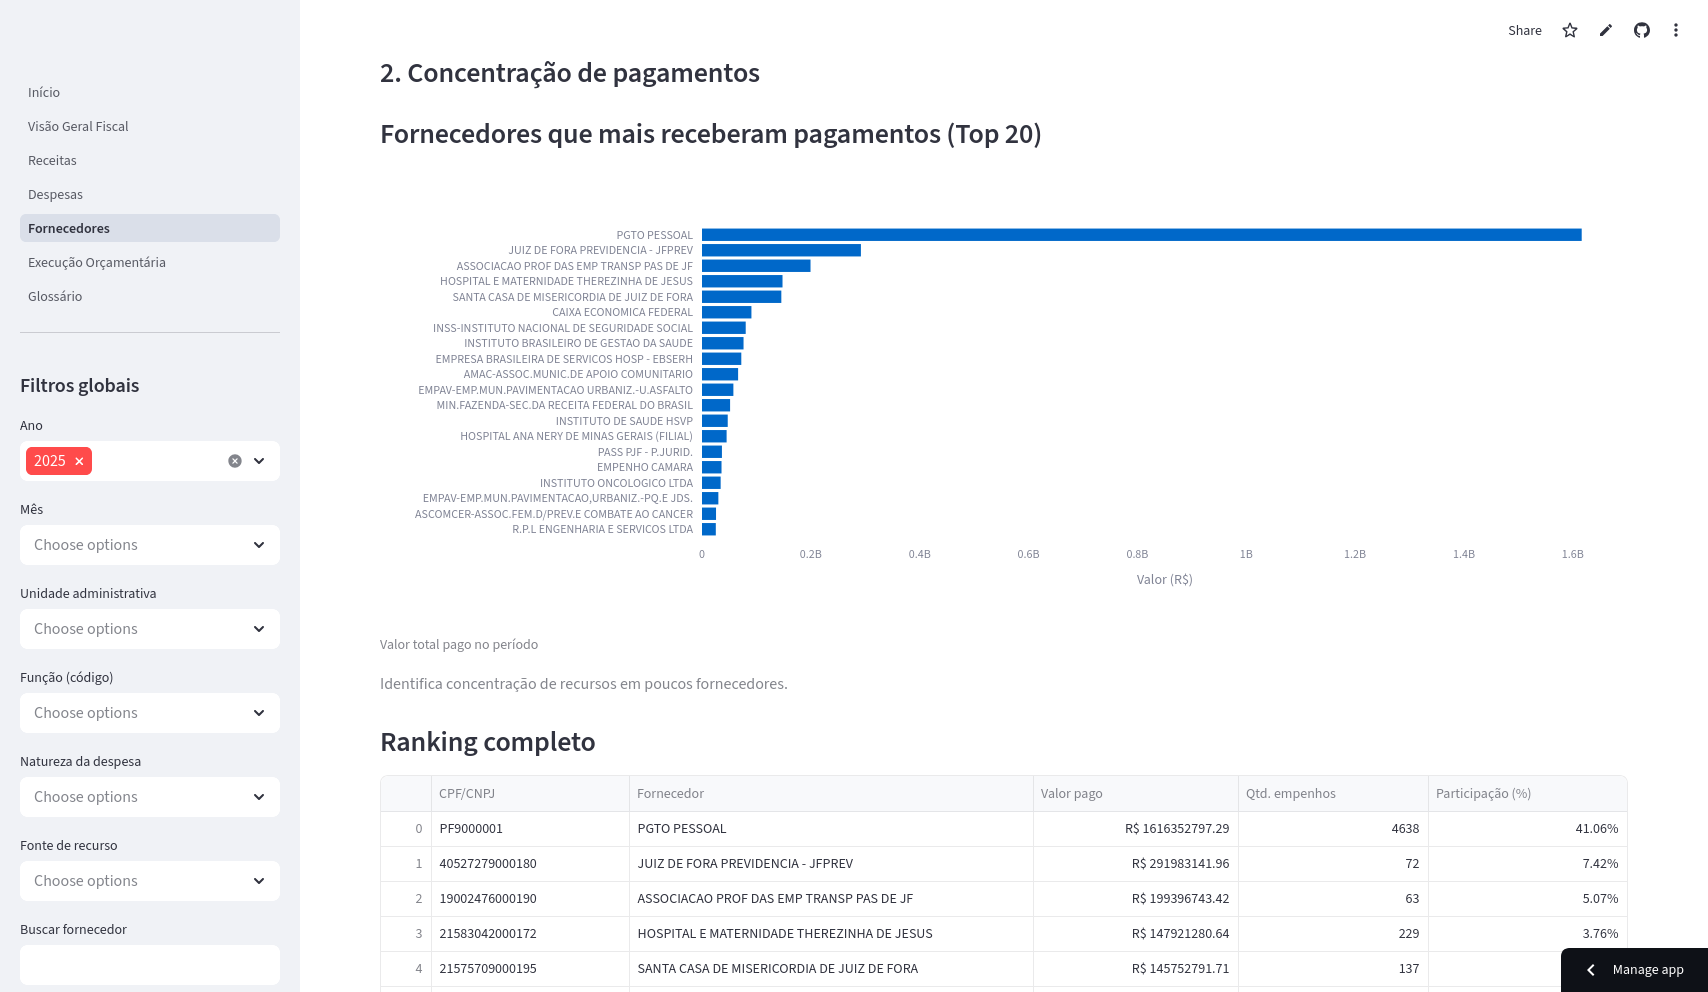
\includegraphics[width=\textwidth]{figs/fornecedores_concentracao.png}
\caption{Fornecedores: concentração de pagamentos (top 20) e ranking completo com participação percentual.}
\label{fig:fornecedores-concentracao}
\end{center}
\end{figure}

\section{Receitas Municipais}

A página Receitas organiza a entrada de recursos. O resumo contrasta previsão atualizada, arrecadação acumulada no recorte, razão realizado/previsão e parcelas classificadas como repasse federal e estadual, utilizando como base prefixos de natureza de receita. A seção "De onde vem o dinheiro" agrupa os códigos MCASP por origem interpretável e exibe barras horizontais por origem. Duas séries temporais comparam previsto e realizado: uma anual (ignorando o filtro de ano, mantendo mês e natureza) e outra mensal. A seção final "Previsto \textit{vs.} realizado" usa uma barra de progresso agregada e uma tabela por natureza de receita, com percentual de realização linha a linha.

Cruzar previsão e arrecadação no portal implica reconciliar arquivos comparativos e de previsão mensal, além de interpretar códigos de natureza sem ementário unificado. O \textit{warehouse} já integra descrições da STN quando disponíveis; o painel traduz a composição da receita em categorias próximas do debate público, o que aproxima o dado da pergunta "de onde vem o dinheiro da cidade?".

\begin{figure}[h]
\begin{center}
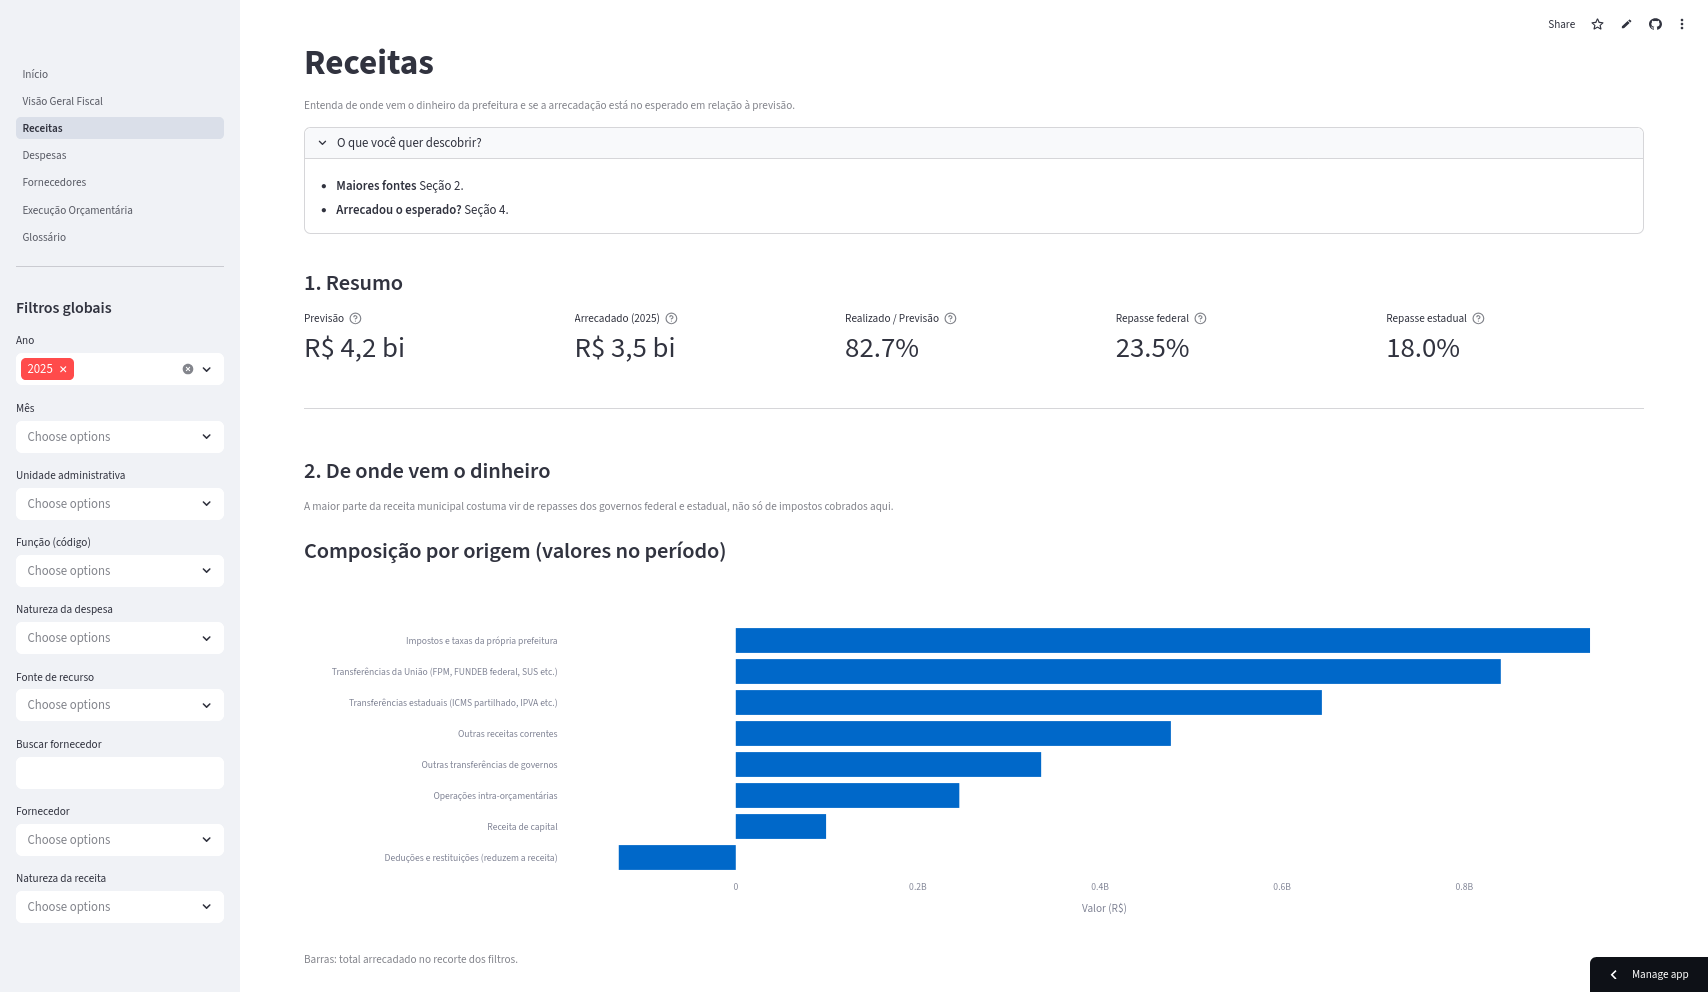
\includegraphics[width=\textwidth]{figs/receitas.png}
\caption{Receitas: resumo do recorte e composição por origem.}
\label{fig:receitas-origem}
\end{center}
\end{figure}

\section{Análise dos Dados de Juiz de Fora}

Descrever painéis não encerra o capítulo de resultados. A proposta do trabalho, ancorada na tradição freireana discutida no Capítulo~\ref{cap:fundamentacao}, exige ir além da descrição da interface e verificar o que o conjunto de números sugere ao ser lido pelo próprio artefato construído. Três padrões emergem da exploração sistemática do \textit{dashboard} sobre a base materializada.

\textbf{Dependência de transferências.} A composição por origem mostra, de forma recorrente, que transferências correntes respondem por parcela expressiva da arrecadação municipal. Isso não é específico de Juiz de Fora, mas torna visível uma premissa muitas vezes invisível no debate local: parte relevante do "orçamento da cidade" depende de repasses cujas regras são definidas fora do município. Um conselheiro ou vereador pode usar o painel para calibrar expectativas sobre o que a prefeitura controla diretamente \textit{vs.} o que é efeito de política nacional ou estadual.

\textbf{Distância entre empenho e pagamento.} Nas páginas de Despesas e Execução Orçamentária, o empenhado tende a superar o liquidado e pago no mesmo recorte quando o período inclui meses recentes do exercício. Isso reflete o ciclo contábil normal, mas também alerta contra leituras simplistas: "gastou" no sentido de empenho não coincide com "saiu do caixa". Restos a pagar e atrasos de liquidação só seriam mensuráveis com granularidade transacional ou com dotação autorizada, limitações já discutidas.

\textbf{Legibilidade funcional incompleta.} Os \textit{fallbacks} de rótulo LOA (Capítulo~\ref{cap:dw}) concentram-se em combinações de menor volume, mas ainda aparecem em cortes que um fiscalizador pode escolher deliberadamente. A análise cidadã ganha densidade quando o leitor combina a tabela funcional com o Glossário e, diante de \texttt{Função XX}, consulta o código ou busca esclarecimento junto ao órgão público.

O que um cidadão pode fazer com essa informação, além de informar-se? Formular perguntas para audiências públicas e sessões de câmara; subsidiar reportagens de jornalismo local com recortes exportáveis da tabela; apoiar entidades do controle social na escolha de prioridades de fiscalização. O painel não substitui um pedido formal de informação nem uma perícia contábil, mas reduz o custo para chegar à primeira evidência quantitativa, passo em que, no portal com dados brutos, muitas pessoas desistem de dar.

Os três padrões descritos acima ilustram o tipo de leitura que o painel viabiliza, mas não esgotam tudo o que ele permite. O Capítulo~\ref{cap:avaliacao} compara, de forma estruturada, o esforço necessário para realizar essas leituras no painel e no portal original.
